% Chapter 1

\chapter{Wearable devices and new human-machine interfaces: an overview}

\lhead{Chapter 1. \emph{Wearable devices and new human-machine interfaces}} % This is for the header on each page - perhaps a shortened title

%----------------------------------------------------------------------------------------

\section{Where to wear an extra eye?}
Positioning an optical device on the human body is quite a problematic task, as occlusion, motion, social issues as well as criteria related to the purpose of the device must be taken into account.\footnote{\url{http://www.robots.ox.ac.uk/~wmayol/3D/nancy_matlab.html}}. Following the work of Mayol \etal \cite{mayol2001positioning}, in this section we give a detailed overview on the best places where to put a wearable camera.

Cameras used for wearable applications fall into two categories for this discussion; static narrow-view devices and omnidirectional devices. Omnidirectional devices include catadioptric, fish-eye and active systems where either the entire field-of-viewis imaged at low resolution, or in the active case the high-resolution narrow-view sensor moved to any orientation. Narrow-view static cameras can only ever see a small part of the user or their environment, and placement is therefore entirely driven by the task. For wide-angle or omnidirectional sensors placement is less constrained and a range of positions are possible. 

A variety of solutions appear in the literature. In \cite{starner1998real, schiele1999attentional}, hat-mounted cameras have been used to look down at the user’s hands and reaching space, whereas in [9, 13] cameras are strapped to the wearer’s hands themselves. In [10], a hat-mounted camera looks forward, an orientation also used when the camera is attached to a head mounted display [2]. In contrast, [11, 6] uses a camera worn on the chest, in [5] an omnidirectional camera is used above the head, and a wide-angle lens camera mounted at the back in [12] and in previous work [4] we placed a miniature active vision system on the shoulder.
In a previous paper [4], we identified three frames of reference for measurements that a wearable sensor makes: I relative to the user body (e.g. sensing the manipulative space in front of the user’s chest) II relative to the static world (e.g. sensing the ceiling/
floor texture to infer user’s location)
III relative to an independent object (e.g. tracking an interesting
object)
This task-oriented classification can help us to understand
the criteria that should be considered. For working
in the user frame alone all that is required is a stable view
of the chosen area — often the handling space, and absolute
field-of-view may be less important. For sensing the
outside environment user occlusion is problematic and absolute
field-of-view is more important. Both occlusion and
user motion are problems when fixating resolution or processing
on a particular part of the environment or independently
moving object.


\begin{figure}[htbp]
	\centering
		\includegraphics[page=3]{Figures/mayol_etal_ouel224101_cropped.pdf}
	\caption[An Electron]{An electron (artist's impression).}
	\label{fig:Electron}
\end{figure}

\begin{figure}[htbp]
	\centering
		\includegraphics[page=4]{Figures/mayol_etal_ouel224101_cropped.pdf}
	\caption[An Electron]{An electron (artist's impression).}
	\label{fig:Electron}
\end{figure}

\begin{figure}[htbp]
	\centering
		\includegraphics[page=5]{Figures/mayol_etal_ouel224101_cropped.pdf}
	\caption[An Electron]{An electron (artist's impression).}
	\label{fig:Electron}
\end{figure}

%----------------------------------------------------------------------------------------

\section{Gestures}
Gestures are expressive, meaningful body motions involving
physical movements of the fingers, hands, arms, head, face, or
body with the intent of conveying meaningful information
or interacting with the environment. They constitute one interesting
small subspace of possible human motion. A gesture
may also be perceived by the environment as a compression
technique for the information to be transmitted elsewhere and
subsequently reconstructed by the receiver. Gesture recognition
has wide-ranging applications such as the following:
\begin{itemize}
\item developing aids for the hearing impaired;
\item  enabling very young children to interact with computers;
\item  designing techniques for forensic identification;
\item recognizing sign language;
\item medically monitoring patients’ emotional states or stress
levels;
\item lie detection;
\item navigating and/or manipulating in virtual environments;
\item communicating in video conferencing;
\item distance learning/tele-teaching assistance;
\item monitoring automobile drivers' alertness/drowsiness
levels, etc.
\end{itemize}

Generally, there exist many-to-one mappings from concepts
to gestures and vice versa. Hence, gestures are ambiguous and
incompletely specified. For example, to indicate the concept
\textit{stop}, one can use gestures such as a raised hand with palm
facing forward, or, an exaggerated waving of both hands over the
head. Similar to speech and handwriting, gestures vary between
individuals, and even for the same individual between different
instances.

Gestures can be static (the user assumes a certain pose or configuration)
or dynamic (with prestroke, stroke, and poststroke
phases). Some gestures also have both static and dynamic elements,
as in sign languages. Again, the automatic recognition
of natural continuous gestures requires their temporal segmentation.
Often one needs to specify the start and end points of a
gesture in terms of the frames of movement, both in time and
in space. Sometimes a gesture is also affected by the context of
preceding as well as following gestures. Moreover, gestures are
often language- and culture-specific. They can broadly be of the
following types:

%----------------------------------------------------------------------------------------

\section{In Closing}
